%% implemen.tex
%% $Id: implemen.tex 4 2005-10-10 20:51:21Z bless $
%%

\chapter{Implementierung}
\label{ch:Implementierung}
%% ==============================
Die Android Applikation, die im Rahmen dieser Arbeit die Daten auf den Smartphones der Probandinnen sammelt, wurde für Android 5.0 "`Lollipop"' implementiert.
Sie kann grob in vier Teilbereiche eingeteilt werden, von denen drei jeweils den entsprechenden zu Sammelnden Daten zugeordnet werden können und das vierte sich mit dem Export der gesammelten Daten beschäftigt.

Da die Applikation darauf ausgelegt ist, nur minimale Interaktion mit der Nutzerin zu haben,
ist das User Interface bewusst minimalistisch gewählt (vergleiche Abbildung \ref{fig:uiscreen}).
Relevant für die Nutzerin sind bei korrekter Ausführung nur die farblich markierten Buttons und das Textfeld am unteren Bildschirmrand.

Die erste Reihe an Buttons dient dazu auch ohne die Möglichkeit Debuglogs zu lesen sicherstellen zu können, dass die Datenbank in der die Applikation die Notifications aufzeichnet nach dem Aufsetzen korrekt arbeitet.
Die Buttons in der zweiten Zeile sind für Verteilen der nichttrivialen Berechtigung, die die Applikation benötigt, durch die Nutzerin bestimmt.
Der große grüne Knopf mit der Aufschrift "`DB Export"' wird von der Nutzerin benutzt sobald die Studie abgeschlossen ist um die gesammelten Daten zu exportieren.
Die Buttons in den Reihen vier und sechs sind wie schon die in der ersten dafür konzipiert, die korrekte Funktionsweise der Applikation zu gewährleisten.
Der mit dem Wort "`Info"' beschriftete Button in der fünften Zeile öffnet das Impressum der Applikation in einem AlertDialog.
Die siebte und unterste Reihe beinhaltet ein Textfeld und einen diesem zugehörigen "`Set Name"' Button.
Mit diesem kann die Nutzerin das von ihr gewählte und auf dem NEO-PI-R Fragebogen aufgeschriebene Pseudonym eintragen und mit dem Button bestätigen um die Zuordnung von Fragenbogen zu Datensatz zu ermöglichen.

\begin{figure}[h]
    \centering
    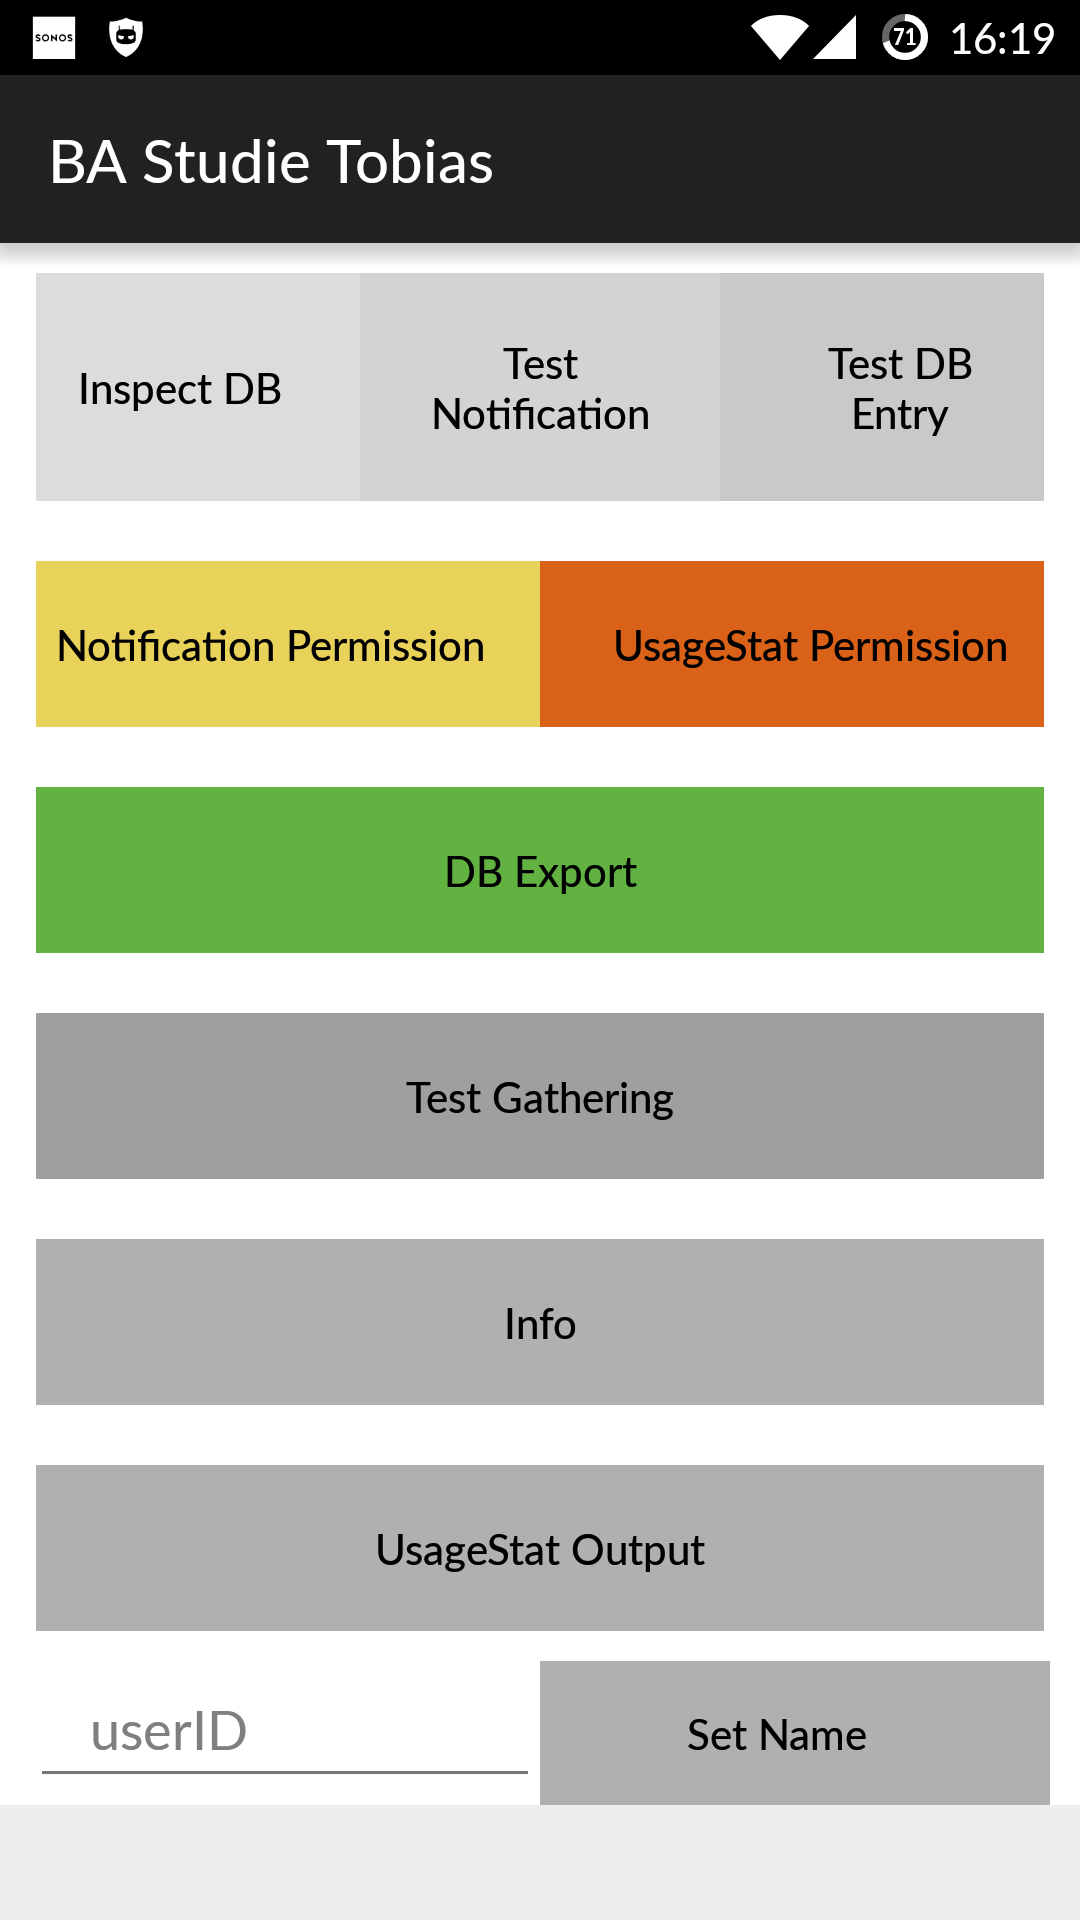
\includegraphics{images/screenshot1.png}
    \caption{User Interface der Applikation}
    \label{fig:uiscreen}
\end{figure}

\section{Call und Message Logs}

Um mit der eigenen Applikation auf die vom Android Betriebssystem gesammelten Logs zu Anrufen und SMS zugreifen zu dürfen müssen die Berechtigungen 
\textbf{android.permission.READ\_CALL\_LOG} und \textbf{android.permission.READ\_SMS} erteilt werden.
Diese können vom Programmierer in der AndroidManifest.xml Datei beantragt werden und da werden, da sie keine besonderen Permissions sind,
von der Nutzerin bei der Installation abgenickt. 
\par
Mit dem Android contentResolver kann nun eine query durchgeführt werden, mit der die Applikation random read access auf die zurückgegebenen Daten erhält.
Über diese Daten kann nun iteriert werden und so die gewünschten Daten extrahiert werden.
Mit jedem weiteren Eintrag wird die gesamte Anzahl und Gesamt dauert inkrementiert und die spezialisierten Aspekte von INCOMING, OUTGOING und MISSED werden per switch case im Falle, dass das aktuelle Item ein ausgehender, ankommender oder verpasser Anruf ist, ebenfalls angepasst.
Die Zählung von einzigartigen Anrufpartnern geschieht hier über eine HashMap, die AnruferID auf einen Integerwert mappt, der bei jedem Auftauchen der AnruferID um eins erhöht wird.
Nachdem so über alle Einträge iteriert wurde, werden die gesammelten Daten in einem CallData Objekt gespeichert.
\par

Die Message Logs verhalten sich bis auf kleine Details, zum Beispiel gibt es keine verpassten SMS, identisch zu den Call Logs und können auf die selbe Weise ausgewertet werden.
Die so gewonnen Daten werden im selben Objekt wie die Daten des Calllogs und werden gemeinsam mit ihnen ausgegeben.



\section{Notification}

\section{NotificationListenerService}
\subsection{Datenbank}

\section{UsageStats}

\section{Export}

Für den Export der gesammelten Daten wird im AndroidManifest.xml die Berechtigung \textbf{android.permission.WRITE\_EXTERNAL\_STORAGE}
benötigt. 
Diese ist keine außergewöhnliche Berechtigung und kann wie die zum Zugang zu Call und Message Log bei der Installation der Applikation beantragt werden.
\par
Die gesammelten Daten werden in drei Dateien in einem eigenen Ordner im \emph{ExternalStorageDirectory} des Smartphones gespeichert werden.
Sie werden als Comma Separated Values (csv) gespeichert.
Die Daten werden in die drei Dateien getrennt nach Notification Daten, Anruf beziehungsweise SMS Daten und UsageStat Daten, um das potenziell automatisierte Auswerten in der Evaluation zu vereinfachen.
Mit Hilfe von OpenCSV, einer einfachen Library zum Lesen und Schreiben von CSV Dateien \cite{opencsv},
wird zunächst die gesamte SQL Tabelle \textbf{TABLE\_NOTIFICATIONENTRIES} zeilenweise in eine Datei geschrieben.
Der Inhalt des callData Objekts wird als String entgegen genommen und nachdem es in einen StringArray gesplittet wurde, spaltenweise in die zweite Datei geschrieben.
In die dritte Datei werden die UsageStat Daten Spaltenweise unter die zugehörigen Package Namen geschrieben.
\par
An alle Dateinamen wird die UserID der Nutzerin, aus der SharedPreference in der sie gespeichert wird, als Suffix angehängt um eine zuordnung der Daten zu den Auswertungsergebnissen der Fragebögen zu ermöglichen.

\section{Probleme bei der Implementierung}
%%% Local Variables: 
%%% mode: latex
%%% TeX-master: "diplarb"
%%% End: 
